\documentclass[]{article}

\usepackage[]{struktex}
\usepackage{graphicx}
\usepackage{lmodern}
\usepackage{svg}

\usepackage[utf8]{inputenc}
\usepackage[T1]{fontenc}
\usepackage[ngerman]{babel}
\usepackage[left=2cm, right=2cm, top=2cm, bottom=2cm, bindingoffset=8mm, includehead, includefoot]{geometry}

% subfigures
\usepackage{caption}
\usepackage{subcaption}

\usepackage{amsfonts}
\usepackage{amssymb}
\usepackage{amsmath}

% Nummerierung mit Alpabet
\usepackage{enumitem}

% paragraph wird wie subsubsection dargestellt und in Inhaltsverzeichnis aufgenommen
\usepackage{titlesec}
\setcounter{secnumdepth}{4}
\setcounter{tocdepth}{4}

\titleformat{\paragraph}
{\normalfont\normalsize\bfseries}{\theparagraph}{1em}{}
\titlespacing*{\paragraph}
{0pt}{3.25ex plus 1ex minus .2ex}{1.5ex plus .2ex}

%opening
\title{Final Task EIB3 WS24|25}
\author{Niklas Bachmann \\ Manuel König}
%\sProofOn
\begin{document}
	
	\maketitle
	%\tableofcontents
	
	\section{Schematics}
		\begin{figure}[htp]
				\centering
				%\includesvg{Proj_scheme.svg}
				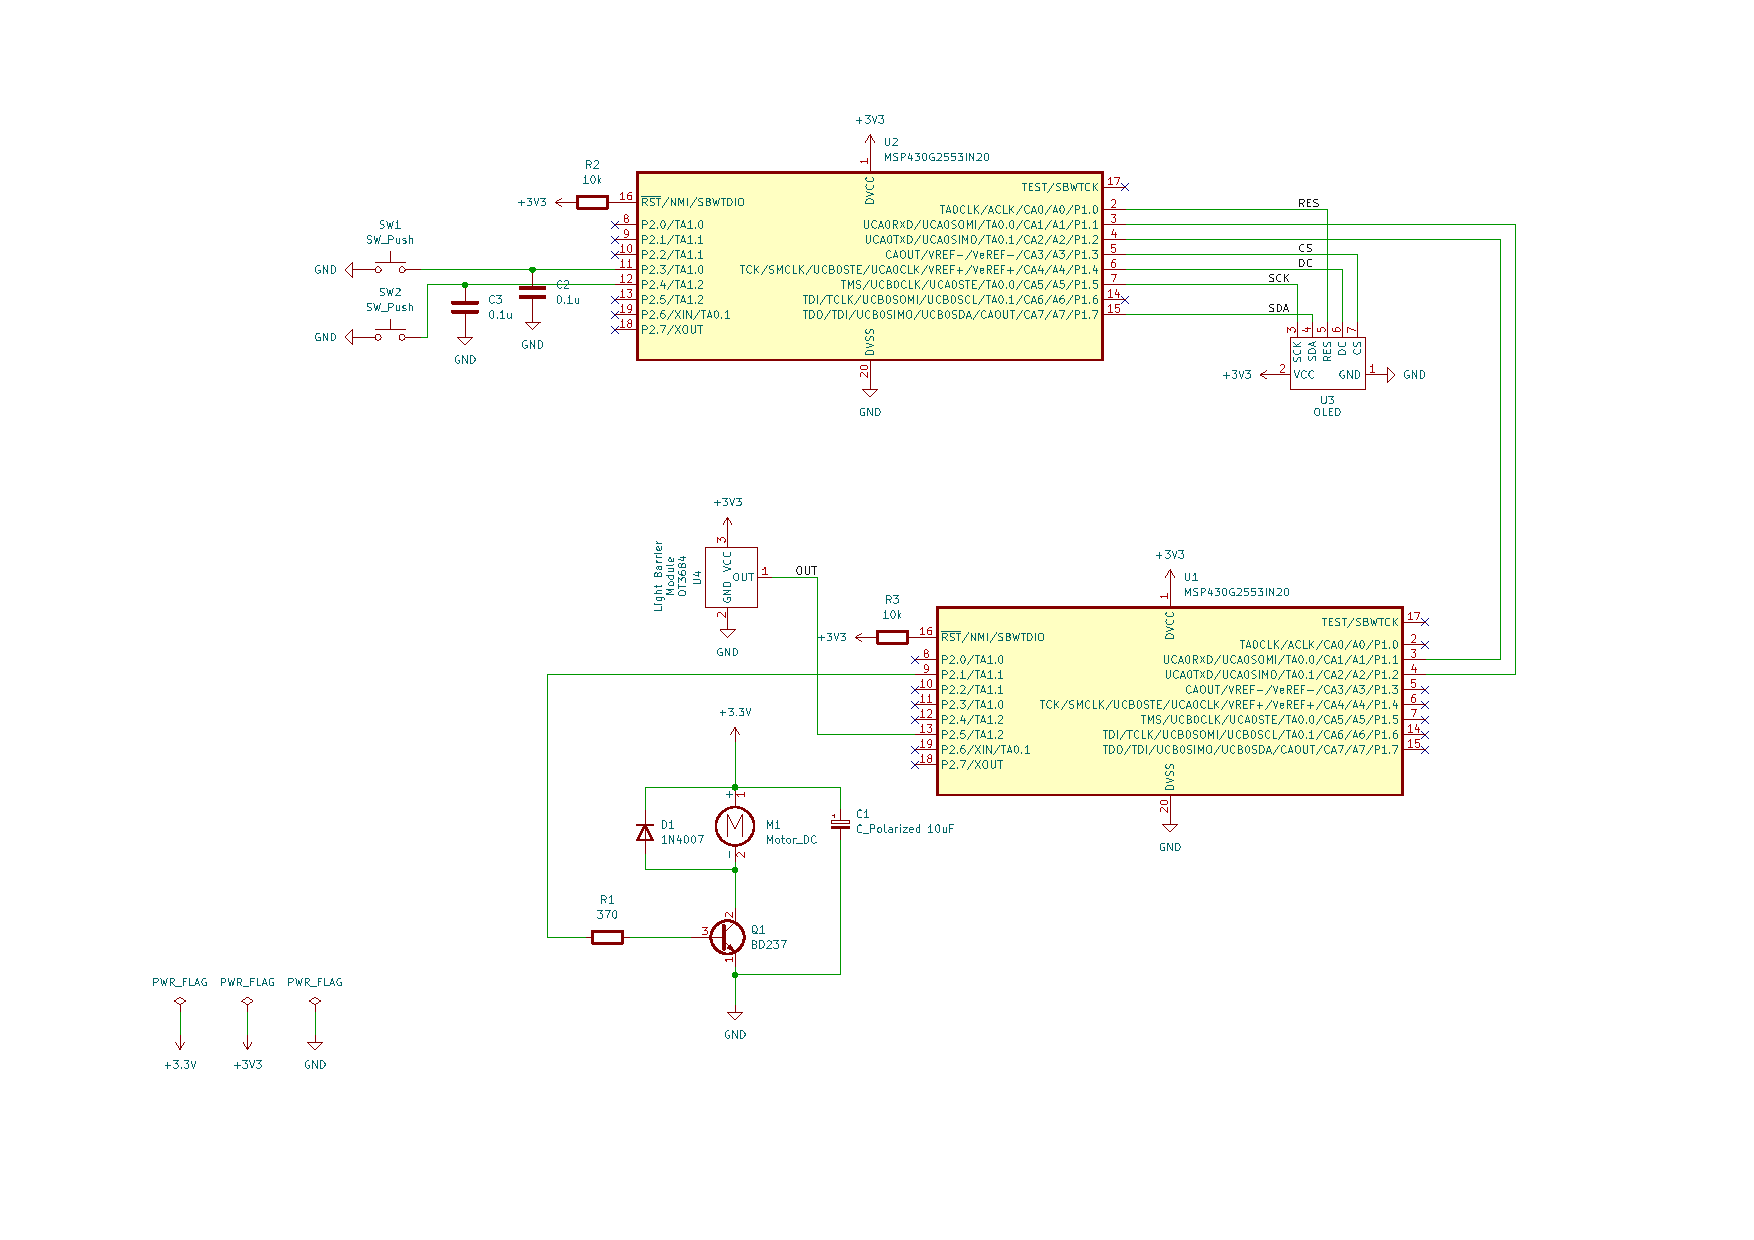
\includegraphics[width=17cm]{Proj_scheme} %[width=9cm, trim=0 2cm 0 0, clip = true]
				\caption{Project scheme}
		\end{figure}
	
	\newpage
	\section{Structograms}
	\subsection{Motor-Controller}
	
	\begin{figure}[htp]
		\centering
		\begin{struktogramm}(160,110)
			\assign{set DCO to 8 MHZ}
			\assign{set Sub- and Main Clock (SMCLK and MCLK) to DCO speed}
			\assign{Initialize UART Interface}
			\assign{Setup Timer0 A0 to trigger Interrupt every x ms}
			\assign{Setup Timer1 A1 to capture light barrier interrupts}
			\assign{enable Interrupts Globaly}
			\assign{get motorSpeed}
			\forever
			\assign{i = position of character in RX Buffer}
			\ifthenelse{7}{1}{i != -1}{yes}{no}
			\assign{create local buffer}
			\assign{copy from RX buffer to local buffer}
			\ifthenelse{7}{1}{i == 6}{yes}{no}
			\assign{encode speed}
			\assign{set motorspeed to new speed}
			\assign{send motorspeed (for debugging)}
			\change
			\ifend
			\change
			\ifend
			\foreverend
		\end{struktogramm}
		\caption{Motor-Controller Main function}
	\end{figure}
	
	\begin{figure}[htp]
		\centering
		\begin{struktogramm}(160,35)
			\ifthenelse{7}{1}{timerDivCounter \textgreater= 7}{yes}{no}
			\assign{send targedSpeed}
			\assign{timerDivCounter = 0}
			\change
			\ifend
			\assign{timerDivCounter++}
		\end{struktogramm}
		\caption{Motor-Controller Timer0\_A0 ISR}
	\end{figure}
	
	\begin{figure}[htp]
		\centering
		\begin{struktogramm}(160,60)
			\assign{calculate interval from TA1CCR2}
			\assign{motorSpeed = $8\cdot 10^6$ / interval}
			\assign{PID routine}
			\ifthenelse{5}{5}{targedSpeed > motorSpeed}{yes}{no}
           		\assign{e = targedSpeed - motorSpeed}
				\assign{e\_sum = e\_sum + e}
				\assign{e\_ld = e - e\_ld}
				\change
				\assign{e = motorSpeed - targedSpeed}
				\assign{e\_sum = e\_sum - e}
				\assign{e\_ld = -e - e\_ld}
			\ifend
			\assign{y = (Kp * e) + (Ki * e\_sum)}
			\assign{limit calculations to uint 16}
			\assign{write PWM value to TA1CCR1}
		\end{struktogramm}
		\caption{Motor-Controller Timer1\_A1 ISR}
	\end{figure}

	%\newline
	\newpage
	
	\subsection{Display-Controller}
	\begin{figure}[htp]
		\centering
		\begin{struktogramm}(160,130)
			\assign{set DCO to 16 MHZ}
			\assign{set Sub- and Main Clock (SMCLK and MCLK) to DCO speed}
			\assign{Initialize UART Interface}
			\assign{Initialize SPI Interface}
			\assign{Initialize and Clear OLED}
			\assign{Setup Timer1 A0 to trigger Interrupt every x ms}
			\assign{Setup DOWN and UP pin to input, pullup, and trigger Interrupt on falling edge}
			\assign{enable Interrupts Globaly}
			\assign{send targedSpeed}
			\assign{update Display}
			\forever
			\assign{i = position of character in RX Buffer}
			\ifthenelse{7}{1}{i != -1}{yes}{no}
			\assign{create local buffer}
			\assign{copy from RX buffer to local buffer}
			\ifthenelse{7}{1}{i == 6}{yes}{no}
			\assign{decode speed}
			\assign{set motorspeed to new speed}
			\assign{send motorspeed (for debugging)}
			\assign{update Display}
			\change
			\ifend
			\change
			\ifend
			\foreverend
		\end{struktogramm}
		\caption{Display-Controller Main function}
	\end{figure}
	
	\begin{figure}[htp]
		\centering
		\begin{struktogramm}(160,35)
			\ifthenelse{7}{1}{timerDivCounter \textgreater= 16}{yes}{no}
			\assign{send targedSpeed}
			\assign{timerDivCounter = 0}
			\change
			\ifend
			\assign{timerDivCounter++}
		\end{struktogramm}
		\caption{Display-Controller Timer1\_A0 ISR}
	\end{figure}
	
	\begin{figure}[htp]
		\centering
		\begin{struktogramm}(160,95)
			\ifthenelse{7}{1}{DOWN}{yes}{no}
			\ifthenelse{4}{4}{targedSpeed \textless \space MINSPEED + INC}{yes}{no}
			\assign{targedSPeed = MINSPEED}
			\change
			\assign{targedSPeed = targedSpeed - INC}
			\ifend
			\change
			\ifend
			\ifthenelse{7}{1}{UP}{yes}{no}
			\ifthenelse{4}{4}{targedSpeed \textgreater \space MINSPEED - INC}{yes}{no}
			\assign{targedSPeed = MAXSPEED}
			\change
			\assign{targedSPeed = targedSpeed + INC}
			\ifend
			\change
			\ifend
			\assign{clear Interrupt}
			\assign{update Display}
		\end{struktogramm}
		\caption{Display-Controller Button UP and DOWN ISR}
	\end{figure}
\end{document}


